\documentclass{article}
\usepackage{amsmath}
\usepackage{MnSymbol}
\usepackage{graphicx}
\usepackage{wasysym}
\usepackage{listings}
\usepackage{color}
\definecolor{mygreen}{RGB}{28,172,0} % color values Red, Green, Blue
\definecolor{mylilas}{RGB}{170,55,241}
\begin{document}
\begin{center}
\LARGE \bfseries{Answers to Problem Set 2}\\
 Group name: Ferienspass\vspace{.5cm}\\
 \normalsize \normalfont
  Sebastian K\"uhnl: 5642348\\
  Alexander D\"uck (as: reebyte): 5504077\\
  Patrick (as: paddyblank): \\
  Christian: 
\end{center}
\normalsize	
	\lstset{language=Matlab,%
		%basicstyle=\color{red},
		breaklines=true,%
		morekeywords={matlab2tikz},
		keywordstyle=\color{blue},%
		morekeywords=[2]{1}, keywordstyle=[2]{\color{black}},
		identifierstyle=\color{black},%
		stringstyle=\color{mylilas},
		commentstyle=\color{mygreen},%
		showstringspaces=false,%without this there will be a symbol in the places where there is a space
		numbers=left,%
		numberstyle={\tiny \color{black}},% size of the numbers
		numbersep=9pt, % this defines how far the numbers are from the text
		emph=[1]{for,end,break},emphstyle=[1]\color{red}, %some words to emphasise
		%emph=[2]{word1,word2}, emphstyle=[2]{style},    
	}
\section*{Question 1}
\subsection*{1.1}
\lstinputlisting{mybisection.m}
\subsection*{1.2}
\lstinputlisting{ffunction.m}
\lstinputlisting{fffunction.m}
\lstinputlisting{PS2P1_2.m}
\subsection*{1.3}
A market equilibrium occurs when markets clear. This implies no excess demand ($D$) or supply ($S$) of Goods. Thus, $q_D = q_S$. This only occurs when $p_D = p_S$ (the market clearing price prevails).
\begin{center} $p_D = p_S$ \end{center}
using
\begin{center} $p_D=a-b*q_D $ and $p_S=c+d*q_S^\psi$\end{center}
 we get
\begin{center} $a-b*q_D =c+d*q_S^\psi$ \end{center}
\begin{center} $0 =c+d*q_S^\psi-(a-b*q_D)$ \end{center}
\begin{center} $0 =c-a+d*q_S^\psi+b*q_D$ \end{center}
\begin{center} $0 =b*q_D+d*q_S^\psi-(a-c)$ \end{center}
Since $q_D = q_S$ holds, this can be written as 
 \begin{equation*} \label{First_One}0=b*q+d*q^\psi-(a-c)\end{equation*} $\blacksquare$\\\\
 a=3, b=0.5, c=d=1, $\psi$=0.5\\\\
 \begin{align*}
 0&=0.5\cdot q+ \sqrt{q}-(3-1) & &\\
 0&=0.5\cdot q+ \sqrt{q}-2 & &\text{substitute:} x^2=q\\
 0&=0.5x^2+x-2&&\text{abc-formula}\\
 x_1&=1.236 &&\text{resubstitution: } q=x^2\\
 x_2&=-3.236&&\text{resubstitution invalid}\\
 \rightarrow q&=\pm 1.112 &&q>0 \\
 \rightarrow q*&=1.112&&\text{insert into: }p=3-0.5q\\
 \rightarrow p*&=2.444&& 
 \end{align*}
\lstinputlisting{demand.m}
\lstinputlisting{supply.m}
\lstinputlisting{difference.m}
\lstinputlisting{PS2P1_3.m}
\section*{Question 2}
\lstinputlisting{PS2P2.m}
\vspace{1cm}
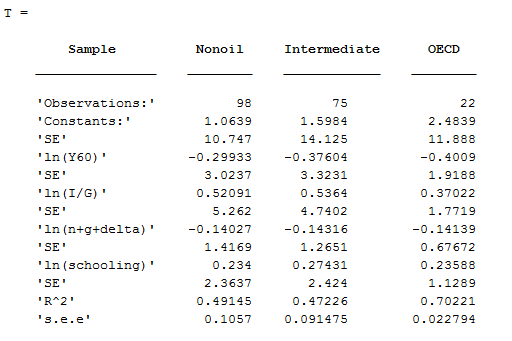
\includegraphics{Table.png}
\end{document}